\documentclass[12pt, titlepage]{article}

\usepackage{booktabs}
\usepackage{tabularx}
\usepackage{hyperref}
\usepackage{soul}
\usepackage{tabularx}
\usepackage{enumerate}
\usepackage{changepage}
\usepackage{graphicx}
\usepackage[utf8]{inputenc}
\usepackage[english]{babel}

\graphicspath{ {./images/} }
\hypersetup{
    colorlinks,
    citecolor=black,
    filecolor=black,
    linkcolor=red,
    urlcolor=blue
}


\title{SE 3XA3: Software Requirements Specification\\KingMe}

\author{Team 9, KingMe
		\\ Ardhendu Barge 400066133
		\\ Dylan Smith 001314410
		\\ Thaneegan Chandrasekara 400022748
}

\date{February 12th, 2021}

\begin{document}

\maketitle

\pagenumbering{roman}
\tableofcontents
\listoftables
\listoffigures

\begin{table}[bp]
\caption{\bf Revision History}
\begin{tabularx}{\textwidth}{p{3cm}p{2cm}X}
\toprule {\bf Date} & {\bf Version} & {\bf Notes}\\
\midrule
7th Feb & 1.0 & Completed section 1\\
11th Feb & 1.1 & Dylan added FR\\
12th Feb & 1.1 & Ardhendu and Thaneegan finished the document\\
\bottomrule
\end{tabularx}
\end{table}

\newpage

\pagenumbering{arabic}


\section{Project Drivers}

\subsection{The Purpose of the Project}
The purpose of this project is to re-implement the checkers game with a Graphical User Interface and adding any missing parts such as proper game instructions. The Artificial Intelligence algorithm for computer play will be optimized for better gameplay and user experience. In addition, missing pieces will be added to make the game regulation size. The game will be reorganized to follow formal software engineering quality attributes.  

\subsection{The Stakeholders}

\subsubsection{The Client}
The client for the checkers game are the teaching staff, specifically the professor and the teaching assistants for the Software 3XA3 course. Throughout the project life-cycle, the client will be involved in providing feedback and reviewing the product implemented. 

\subsubsection{The Customers}
The customers for the checkers game include anyone who is interested in learning how to play, or anyone looking to improve their existing skills or just enjoy the game.

\subsubsection{Other Stakeholders}
In addition to the client and customers specified above, another group of stakeholders include chess organizations and developers who will work on this open-source project in the future. Checkers organizations can range from school clubs to professional clubs that are looking to transition in-person play to online. Future developers are an indirect stakeholder group, as they will be interested in developing a well-documented, logical project.

\subsection{Mandated Constraints}
\begin{itemize}
    \item The checkers game will be based on the open source project by codeofcarson.
    \item The project must be completed by April 12 2021.
    \item The project must be able to run on the McMaster Mills server.
    \item The budget for the project is \$0, which will affect the quality of product being developed.
\end{itemize}
\subsection{Naming Conventions and Terminology}
\begin{itemize}
    \item GUI: Graphical User Interface
    \item AI: Artificial Intelligence
    \item UI: User Interface
\end{itemize}

\subsection{Relevant Facts and Assumptions}
\subsubsection{Facts}
\begin{itemize}
    \item The existing open-source project does not have certain checkers rules implemented.
    \item The existing open-source project is a smaller version of checkers that does not have all the pieces and is played on a smaller board.
    \item The existing open-source project has 388 lines of code.
\end{itemize}
\subsubsection{Assumptions}
\begin{itemize}
    \item The user has a device to play the chess game on.
    \item The user's device has Python downloaded in order to run the application.
    \item The user is capable of reading English and following instructions written in English.
    \item User is able to use computer and internet
\end{itemize}

\section{Functional Requirements}

\subsection{The Scope of the Work and the Product}
The software product being built is a command line versions of the game of checkers. The game will be improved from its previous version by updating it to include all 24 checkers pieces as opposed to the 12 pieces currently implemented. The checkers game will be implemented to follow all the rules of checkers, a tutorial will be made available to users to help beginners learn how the rules. A Graphical User Interface will also be added to improve the playability of the game. If time permits alternate versions of checkers will be added to make the app appeal to more people.
\subsubsection{The Context of the Work}
The context of the checkers app is going to be a command line application. It will be made using the python programming language. External libraries such as pygame will be used to help developers with the construction of the Graphical User Interface.
\subsubsection{Work Partitioning}

\begin{table}[h!]
    \begin{center}
	\caption{\bf Work Partitioning}
	\begin{adjustwidth}{-1.5cm}{}
	\begin{tabularx}{1.2\textwidth}{p{2.5cm}p{2.1cm}p{3.4cm}X}
		\toprule {\bf Event Name}  & {\bf Input} & {\bf Output} & {\bf Description} \\
		\midrule
		Start Game & User Input & State creation, Graphic creation, Display change & User starts game and system outputs the initial state of the board\\
		View Tutorial & User Input & Graphic creation, Display change & User clicks on tutorial and the system outputs the rules of checkers\\
		Make a move & User Input & State creation, Graphic creation, Display change, AI & When a user makes a move the system will update and display the board and then the AI will make a move \\
		Leave game & User Input & Graphic creation, Display change & User chooses to leave game and the system returns to the home screen\\
		\bottomrule
	\end{tabularx}
	\end{adjustwidth}
	\end{center}
\end{table}

\subsubsection{Individual Product Use Cases}
    \textbf{Case UC-1}: Play ckeckers\\
    \textbf{Related Requirements}: FR1-FR9\\
    \textbf{Initiating Actor}: The user\\
    \textbf{Actor's Goal}: Play a game of checkers.\\
    \textbf{Participating Actors}: None\\
    \textbf{Preconditions}: No game is in progress, system is displaying the home screen.\\
    \textbf{Postconditions}: Either the win or loss state is achieved\\
    \textbf{Flow of Events for Main Success Scenario}:\\
    $\rightarrow$ 1. The initiating user chooses to start a game.\\
    $\leftarrow$ 2. System prompts user to choose their opponent (either the computer or another player).\\
    $\rightarrow$ 3. The user chooses their opponent.\\
    $\leftarrow$ 3.1 If the user chooses to play the computer the system prompts them to choose the colour of their pieces.\\
    $\rightarrow$ 3.2 User chooses their colour (if they chose to play the computer).\\
    $\leftarrow$ 4. System displays the state of the board.\\
    $\leftrightarrow$ 5. The player with the black pieces moves first.\\
    $\leftarrow$ 6. The system updates the state of the board.\\
    $\leftrightarrow$ 7. The player with the red pieces moves next.\\
    $\leftarrow$ 8. The system updates the state of the board.\\
    $\leftarrow$ 9. Players alternate turns until a win/loss state is achieved.\\
    \textbf{Flow of Events for Alternative Scenarios}:\\
    \textbf{Leave game:}\\
    $\leftarrow$ 1. The user chooses to leave the current game.\\
    $\rightarrow$ 2. The system returns to home screen.\\
    \textbf{Invalid move:}\\
    $\leftarrow$ 1. The user attempts to make an invalid move.\\
    $\rightarrow$ 2. The system displays and error message.\\
    $\rightarrow$ 3. The system returns the state of the board to what it was before the invalid move was attempted.
    
    
\subsection{Functional Requirements}
Rules of the checkers game were referred to via \cite{CheckersWikipedia}
\begin{enumerate}[{FR}1.]
    \item\textbf{Description}: The system shall have a home screen that provides option to user to start a game or view the checkers tutorial.\\
        \textbf{Rationale}: System shall allow the user to start a game or view the tutorial whenever they want.\\
        \textbf{Fit Criterion}: The system remains on the home screen until the user initiates an event.\\
        \textbf{Originator}: Dylan Smith added February 11, 2021.
        
    \item\textbf{Description}: The system will allow the user to choose their colour.\\
        \textbf{Rationale}: To give the user the option to play first or second.\\
        \textbf{Fit Criterion}: When the user selects the "1-Player" mode the system waits for the user to choose their colour.\\
        \textbf{Originator}: Dylan Smith added February 11, 2021.
        
    \item\textbf{Description}: The system will only allow the User/AI to make valid moves.\\
        \textbf{Rationale}: To abide by the rules of checkers.\\
        \textbf{Fit Criterion}: The User/AI can only choose from a set of valid squares.\\
        \textbf{Originator}: Dylan Smith added February 11, 2021.
        
    \item\textbf{Description}: The system will show all valid moves for the piece the user selects.\\
        \textbf{Rationale}: This will help the user find valid moves if they are just learning how to play. \\
        \textbf{Fit Criterion}: When the user selects a piece to move the system displays all valid moves.\\
        \textbf{Originator}: Dylan Smith added February 11, 2021.
        
    \item\textbf{Description}: The system shall display an error message if an invalid move is attempted.\\
        \textbf{Rationale}: The user needs to know that the move they attempted is invalid, that it won't be accepted, and that it remains their turn.\\
        \textbf{Fit Criterion}: An error message is displayed when an invalid move is made.\\
        \textbf{Originator}: Dylan Smith added February 11, 2021.
        
    \item\textbf{Description}: The system shall display the state of the board after each move.\\
        \textbf{Rationale}: The user will need a way to keep track of the moves that have been made.\\
        \textbf{Fit Criterion}: When a move is made the system will display the move on the board.\\
        \textbf{Originator}: Dylan Smith added February 11, 2021.
        
    \item\textbf{Description}: The system shall provide users with the option to leave the current game.\\
        \textbf{Rationale}: The user may have chosen "1-Player" and may wish to change to "2-Player mode without having to play the game to completion.\\
        \textbf{Fit Criterion}: The system provides the user with the option to leave the game and return to the home screen.\\
        \textbf{Originator}: Dylan Smith added February 11, 2021.
        
    \item\textbf{Description}: The user shall win once it captures all the pieces of the opponent.\\
        \textbf{Rationale}: Signifies the win state for user.\\
        \textbf{Fit Criterion}: All of the opponents pieces have been removed from the board.\\
        \textbf{Originator}: Ardhendu added February 12, 2021.
        
    \item\textbf{Description}: The user shall lose once opponent captures all the pieces of the user.\\
        \textbf{Rationale}: Signifies the loss state for user.\\
        \textbf{Fit Criterion}: All of the users pieces have been removed from the board.\\
        \textbf{Originator}: Ardhendu added February 12, 2021.
        
    \item\textbf{Description}: The system will display a win/loss screen when a win/loss state is achieved.\\
        \textbf{Rationale}: To signify the end of the game.\\
        \textbf{Fit Criterion}: The system displays the win/loss screen when a final state is reached.\\
        \textbf{Originator}: Dylan Smith added February 11, 2021.
    
     \item\textbf{Description}: The system must remove a user/opponents piece when it is jumped over by another piece.  \\
        \textbf{Rationale}: To display the correct state of the game.\\
        \textbf{Fit Criterion}: The piece that was jumped over will no longer appear on the board.\\
        \textbf{Originator}: Thaneegan added February 12, 2021.
        
    \item\textbf{Description}: User can only control their pieces during their turn.\\
        \textbf{Rationale}: To prevent user from controlling opponents pieces. \\
        \textbf{Fit Criterion}: The user is not active during the opponent's turn. \\
        \textbf{Originator}: Thaneegan added February 12, 2021.  
        
    \item\textbf{Description}: Black side shall be the first one to move a piece.\\
        \textbf{Rationale}: To abide by the game rules.\\
        \textbf{Fit Criterion}:  Only black side will be able to choose pieces on the first turn.\\
        \textbf{Originator}: Ardhendu added February 12, 2021 
        
    \item\textbf{Description}: Any piece on the board shall not move backwards except king piece\\
        \textbf{Rationale}: To abide by the game rules. \\
        \textbf{Fit Criterion}: When the user selects a non-king piece to move, the system only allows forward moves.\\
        \textbf{Originator}: Ardhendu added February 12, 2021 
    
    \item\textbf{Description}: Pawn piece shall be promoted to king piece if it makes to opposite side of the board\\
        \textbf{Rationale}: To abide by the game rules.\\
        \textbf{Fit Criterion}: Pawn piece replaced by king piece on board. \\
        \textbf{Originator}: Thaneegan added February 12, 2021.
        
    \item\textbf{Description}: A piece selected by the user shall be highlighted.\\
        \textbf{Rationale}: To provide the user with a visual that a piece has been selected.\\
        \textbf{Fit Criterion}: The desired piece has been highlighted. \\
        \textbf{Originator}: Thaneegan added February 12, 2021.
        
\end{enumerate}

\section{Non-functional Requirements}

\subsection{Look and Feel Requirements}
\begin{itemize}
    \item The game shall be visually appealing to 90\% of users or more.
    \item The game display shall be able to scale in size as the user desires.
\end{itemize}

\subsection{Usability and Humanity Requirements}
\begin{itemize}
    \item The game will be usable by users with color blindness.
    \item The game will be usable by users who can operate a computer.
    \item The game shall have a tutorial for new users to learn the rules.
\end{itemize}

\subsection{Performance Requirements}
\begin{itemize}
    \item The game must move a user's piece within 2 seconds of the user requesting that move.
    \item The game must move a computer's piece within 3 seconds of the user completing their turn.
    \item The game must be started and displayed within 5 seconds of the user requesting to play a game.
    \item The game shall run at a frame rate of 60 frames per second or above.
\end{itemize}

\subsection{Operational and Environmental Requirements}
\begin{itemize}
    \item The user must have python installed on their device.
    \item The game shall run on the user's device without the need for internet.
\end{itemize}

\subsection{Maintainability and Support Requirements}
\begin{itemize}
    \item The game shall be well documented.
    \item The game must be modularized into different components.
    \item The code must follow same coding style throughout. 
\end{itemize}

\subsection{Security Requirements}
\begin{itemize}
    \item The game must not request the user for personal information.
    \item The game must not request the user to download nor install anything.
\end{itemize}

\subsection{Cultural Requirements}
\begin{itemize}
    \item N/A
\end{itemize}

\subsection{Legal Requirements}
\begin{itemize}
    \item The game must not use any symbols that are owned by other creators.
\end{itemize}

\subsection{Health and Safety Requirements}
\begin{itemize}
    \item N/A
\end{itemize}
\section{Project Issues}

\subsection{Open Issues}
There are several existing issues with the original implementation that significantly impact the ability to play and enjoy the game:
\begin{itemize}
\item The lack of a GUI results in a poor appearance to the user. Instead of having a user-friendly GUI, the original implementation forces the user to use the command-line interface to make moves. This affects not only appearance but also performance as well.
\item The original implementation is not intuitive as the game does not have sufficient instructions nor rules to help the user understand the game.
\item The game does not run on devices with python versions 3.x.x, and instead only run on devices with older versions of python installed such as the python 2.x.x versions. This impacts the usability of users wishing to play the game and acts as a barrier to entry for those who do not wish to install an older version of python.
\item The game does not use the standard checkers board or the standard number of pieces. This limited version of checkers will limit interest from users.
\end{itemize}
\subsection{Off-the-Shelf Solutions}
Checkers is a very popular game and thus there exists multiple online or downloadable versions. Each off-the-shelf solutions varies in detail, but the core revolves the same rules of checkers. The following are a few examples of checkers games online:
\begin{itemize}
    \item \href{https://cardgames.io/checkers/}{https://cardgames.io/checkers/}
    \item \href{https://www.gametop.com/download-free-games/checkers/}{https://www.gametop.com/download-free-games/checkers/}
    \item \href{https://www.247checkers.com/}{https://www.247checkers.com/}
    \item \href{https://www.malavida.com/en/soft/checkers-deluxe/#gref}{https://www.malavida.com/en/soft/checkers-deluxe/#gref}
    \item \href{https://gametable.org/games/checkers/}{https://gametable.org/games/checkers/}
\end{itemize}
There are also solutions that are available on GitHub pages or PyPi to download and play. An example of this can be seen below:
\begin{itemize}
    \item \href{https://pypi.org/project/imparaai-checkers/}{https://pypi.org/project/imparaai-checkers/}
\end{itemize}
\subsection{New Problems}
As describe in section 4.1 (open issues), there are several issues with the original implementation. As these issues are worked on and fixed, new issues may arise. Although we plan on implementing the best solution possible, there may be a few hypothetical new problems that occur:
\begin{itemize}
    \item The transition from the original implementation's command-line interface UI to a GUI instead may result in performance issues. Although we aim to have quick performance, as mentioned in our NFRs, the use of a GUI will increase the response time required and we will have to implement an efficient algorithm to prevent this  problem from arising.
    \item Another problem that may arise after introducing a GUI is not displaying the GUI properly due to various user screen sizes. The GUI must be flexible and stretchable in both X and Y directions such that the resolution of the images/components on screen do not look worse. Although we will implement the solution to avoid this problem, time may be a constraint in testing for this.
\end{itemize}

\subsection{Tasks}
The tasks for this project are specified by the stakeholder Dr.Bokhari. These tasks, along with the deadline dates, can be found on our Gantt tasks chart available here: \href{https://gitlab.cas.mcmaster.ca/bargea/3xa3-g09-2021/-/blob/master/BlankProjectTemplate/ProjectSchedule/3XA3\%20Group\%20Project.pdf}{Project Tasks}. The Gantt task chart can also be viewed down below: 
\begin{figure}[h]
    \centering
    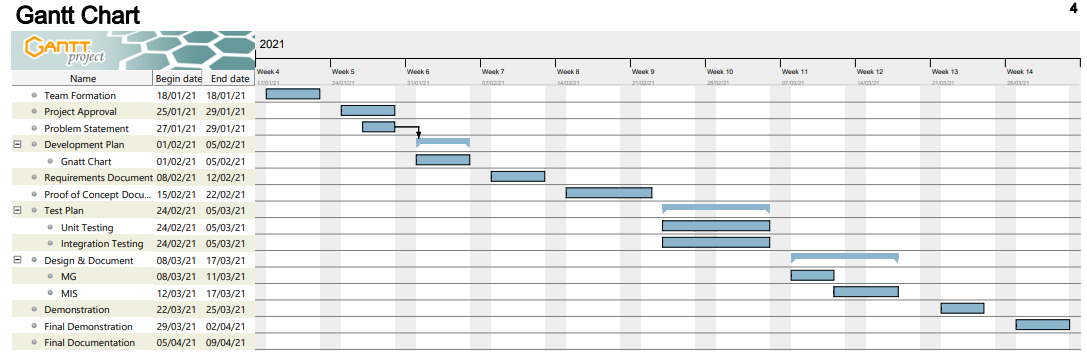
\includegraphics[scale=0.55]{GanttChart}
    \caption{Project Gantt Chart}
    \label{fig:GanttChart}
\end{figure}


\subsection{Migration to the New Product}
The current open-source project supports Python version 2.x.x but does not support Python 3.x.x. Thus we will be migrating the existing code to Python 3 to resolve this.

\newpage
\subsection{Risks}
\begin{table}[h!]
\centering
\begin{tabular}{ |p{7cm}|p{3cm}|p{3cm}| } 
\hline
Risk & Probability of Occurring & Level of impact \\
\hline
Testing does not discover all errors/bugs that were made during development before production release. & High & Medium \\ 
\hline
The GUI developed does not adjust accordingly when the user stretches the GUI in the X or Y directions. & Medium & Medium \\
\hline
Response time (as specified in NFRs) is not met successfully. & Medium & Low \\ 
\hline
Transition from supporting Python 2 to Python 3 is not completed. & Low & Low \\ 
\hline
\end{tabular}
\end{table}

\subsection{Costs}
There is no monetary costs involved in this version of the project. The features being added to the existing open-source project do not require any money nor do any of the team-members require compensation. 
However in terms of cost of effort/time, the project Gantt chart illustrates the distribution of work among the team resources. Please refer to our Gantt resource chart for this project here: \href{https://gitlab.cas.mcmaster.ca/bargea/3xa3-g09-2021/-/blob/master/BlankProjectTemplate/ProjectSchedule/3XA3\%20Group\%20Project.pdf}{Project Schedule}.

\subsection{User Documentation and Training}
User documentation and training will come in the form of two methods:
\begin{itemize}
    \item Walk-through tutorial: The walk-through tutorial will be an optional explanation on how to play the game and where various buttons are on the UI.
    \item Rules page: There will also be an option for the user to click to view/read the rules of checkers on their own.
\end{itemize}
\subsection{Waiting Room}
There are a few requirements that are on the waiting list to be included in future versions:
\begin{itemize}
    \item Difficulty of Opponent: A feature to allow the user to select difficulty of opponent (computer). There would be a range of difficulty levels to accommodate for different users with different skill-levels ranging from beginner to expert. Currently time constraint prevents us from implementing this feature.
    \item Multiplayer: A feature to allow the user to play online against other human-players rather than just against the computer. Currently budget and time constraints prevent us from implementing this feature.
    \item Advertisements: In order to bring in revenue for the game, a feature to be added in the future would be advertisements. These advertisements would be displayed either before the game begins for a set amount of time, or displayed on the sides of the screen. Currently time constraints prevent us from incorporating this.
\end{itemize}

\subsection{Ideas for Solutions}
The following points below indicate how we will approach the design/implementations for the code:
\begin{itemize}
    \item Pygame will be used to implement the checkers game. Although there are various other libraries that could be used, Pygame is perfect for games that are not movement-intensive and for games that do not require high resolution to play.
    \item Pygame GUI is a useful module that will help us create the GUI. It is open-source and the only dependency is Pygame.
\end{itemize}

\newpage

\section{Appendix}
N/A

\subsection{Symbolic Parameters}
N/A
\bibliographystyle{plain}
\bibliography{SRS.bib}


\end{document}